\uuid{Odn4}
\niveau{PCSI}
\module{Analyse}
\chapitre{Convergence d'une suite}
\sousChapitre{Suite, monotonie et point fixe}
\duree{30}
\difficulte{1}
\auteur{Antoine Crouzet}
\datecreate{01/12/2024}
\titre{Suites et point fixe II}
\contenu{
\texte{On considère la fonction $f$ définie sur $\R$ par : $f(x)=\dfrac{1}{2}x^2-\dfrac{3}{2}x+3$ ; ainsi que la suite $(u_n)_{n\geq 0}$
définie par : $u_0=2,5$ et, pour tout $n\geq 0$, $u_{n+1}=f(u_n)$.}
\question{Mettre $f(x)$ sous forme canonique.}
\reponse{\label{td11-9-q1} Pour tout réel $x$, on constate que :
		\begin{align*}
			f(x) &= \frac{1}{2}(x^2-3x) + 3\\
			     &= \frac{1}{2}\left( \left(x-\frac32\right)^2 - \frac94\right) + 3 \\
				 &= \frac12 \left(x-\frac32\right)^2 - \frac{9}{8}+3\\
				 &= \frac12 \left(x-\frac32\right)^2 +\frac{15}{8}
		\end{align*}}
\question{Montrer que l'intervalle $[2,3]$ est stable par $f$.}
\reponse{\label{td11-9-q2} On utilise la relation de la question \ref{td11-9-q1}. Soit $x\in [2;3]$. Alors
		\begin{align*}
		   2 \leq x \leq 3 &\implies \frac12 \leq x-\frac{3}{2}\leq \frac32\\
		   				   &\implies \frac14 \leq \left(x-\frac32\right)^2 \leq \frac94 \text{ car la fonction carrée est croissante sur }\R+\\
						   &\implies \frac18 \leq \frac{1}{2}\left(x-\frac32\right)^2 \leq \frac98 \\
						   &\implies 2=\frac{16}{8}\leq  \frac12 \left(x-\frac32\right)^2 +\frac{15}{8} \leq \frac{24}{8}=3
		\end{align*}
		Ainsi, pour tout réel $x\in [2;3]$, $f(x)\in [2;3]$ : l'intervalle $[2;3]$ est stable par $f$.}
\question{Montrer que pour tout $n\geq 0$, $u_n\in [2;3]$.}
\reponse{\begin{align*}
\label{td11-9-q3} Soit $P$ la proposition définie pour tout entier $n$ par $P_n$: ``$u_n\in [2;3]$''.
		\begin{description}
			\item \textbf{Initialisation} : pour $n=0$, $u_0=2,5\in[2;3]$ : $P_0$ est vraie.
			\item \textbf{Hérédité} : supposons la proposition $P_n$ vraie pour un certain entier $n$ fixé, et démontrons que $P_{n+1}$ est vraie.\\Ainsi, par hypothèse de récurrence, $u_0\in [2;3]$. Or, on a montré à la question \ref{td11-9-q2} que l'intervalle $[2;3]$ est stable par $f$. Donc, puisque $u_n\in[2;3]$, $f(u_n)\in [2;3]$, c'est-à-dire $u_{n+1}\in [2;3]$ : la proposition $P_{n+1}$ est donc vraie et la propriété est héréditaire.
		\end{description}
		D'après le principe de récurrence, la proposition $P_n$ est vraie pour tout entier $n$, c'est-à-dire : \[ \boxed{\forall~n\in \N,\quad u_n\in[2;3]}\]
\end{align*}}
\question{\'Etudier le signe de $f(x)-x$.}
\reponse{\label{td11-9-q4} Fixons un réel $x$. On a alors 
		\begin{align*}
			f(x)-x &= \frac12 x^2 -\frac32x +3 - x \\
				   &= \frac12 x^2 -\frac52x + 3
		\end{align*}
		On dresse le tableau de signe de ce trinôme du second degré : le discriminant vaut $\Delta = \frac14$ et les racines sont donc $x_1=2$ et $x_2=3$. On obtient le tableau de signe suivant :
\begin{center}  \begin{tikzpicture}
           \tkzTabInit[lgt = 2, espcl = 1.5]{$x$ / 1 , $f(x)-x$ / 1}{$-\infty$, $2$, $3$, $+\infty$}
           \tkzTabLine{,+,z,-,z,+,}
        \end{tikzpicture}
\end{center}}
\question{\'Etudier le sens de variation de $(u_n)_{n\geq 0}$.}
\reponse{\begin{align*}
\label{td11-9-q5} On utilise les questions \ref{td11-9-q3} et \ref{td11-9-q4}. Pour tout entier $n$, $u_n\in [2;3]$. Or, on vient de voir que si $x\in [2;3]$, $f(x)-x\leq 0$. Ainsi, pour tout entier $n$, $f(u_n)-u_n\leq 0$, c'est-à-dire $u_{n+1}-u_n\leq 0$ : la \fbox{suite $(u_n)$ est décroissante.}.
\end{align*}}
\question{Montrer que $(u_n)_{n\geq 0}$  est convergente puis déterminer sa limite.}
\reponse{\begin{align*}
D'après la question \ref{td11-9-q5}, la suite $(u_n)$ est décroissante. D'après la question \ref{td11-9-q2}, elle est minorée par $2$. D'après le théorème de la limite monotone, on en déduit que la suite $(u_n)$ est convergente.\\
		Notons $\ell$ sa limite. Par somme et produit, on a \[ \frac12 u_n^2-\frac32 u_n+3 \tendversen{n\to+\infty} \frac12 \ell^2-\frac32 \ell+3 \]
		De plus, $\ds{\lim_{n\to+\infty} u_{n+1} = \lim_{n\to +\infty}u_n=\ell}$. En utilisant la définition de la suite $u$, on a \[ u_{n+1}=\frac12 u_n^2 -\frac32u_n+3 \]
		et par passage à la limite \[ \ell = \frac12 \ell^2-\frac32\ell +3 \]
		c'est-à-dire $\frac12\ell^2-\frac52\ell+3=0$, équation déja résolue dans la question \ref{td11-9-q4}, et qui admet comme solutions $2$ et $3$. Or, la suite $(u_n)$ est décroissante, et $u_0=2,5$; elle ne peut donc pas converger vers $3$. On en déduit finalement que \[ \boxed{\lim_{n\to +\infty} u_n = 2} \]
\end{align*}}
}
